 \documentclass{article}
\usepackage{graphicx}
\usepackage[utf8]{inputenc}
\usepackage{listings}
\usepackage{color}
\usepackage{xcolor}
\usepackage{textcomp}
\usepackage{amsmath}
\usepackage{mathabx}

\definecolor{solarized@base03}{HTML}{002B36}
\definecolor{solarized@base02}{HTML}{073642}
\definecolor{solarized@base01}{HTML}{586e75}
\definecolor{solarized@base00}{HTML}{657b83}
\definecolor{solarized@base0}{HTML}{839496}
\definecolor{solarized@base1}{HTML}{93a1a1}
\definecolor{solarized@base2}{HTML}{EEE8D5}
\definecolor{solarized@base3}{HTML}{FDF6E3}
\definecolor{solarized@yellow}{HTML}{B58900}
\definecolor{solarized@orange}{HTML}{CB4B16}
\definecolor{solarized@red}{HTML}{DC322F}
\definecolor{solarized@magenta}{HTML}{D33682}
\definecolor{solarized@violet}{HTML}{6C71C4}
\definecolor{solarized@blue}{HTML}{268BD2}
\definecolor{solarized@cyan}{HTML}{2AA198}
\definecolor{solarized@green}{HTML}{859900}

\lstset{
  language=Java,
  upquote=true,
  columns=fixed,
  tabsize=2,
  extendedchars=true,
  breaklines=true,
  frame=single,
  numbers=left,
  numbersep=5pt,
  rulesepcolor=\color{solarized@base03},
  numberstyle=\tiny\color{solarized@base01},
  basicstyle=\footnotesize\ttfamily,
  keywordstyle=\color{solarized@green},
  stringstyle=\color{solarized@cyan}\ttfamily,
  identifierstyle=\color{solarized@blue},
  commentstyle=\color{solarized@base01},
  emphstyle=\color{solarized@red}
}
\begin{document}

\title{Tarea Método de falsa posicion}
\author{Angel Caceres Licona}

\maketitle


\section{Considere la función $f(x) = x^2 -4\cos(x)$...}

\subsection{Graficar en el intervalo $(1,2)$...}


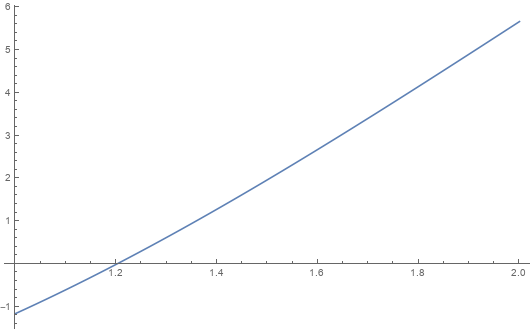
\includegraphics[scale=0.4]{graficaFalsa1.png}



\section{Código del programa}

\begin{lstlisting}
from math import *

def fx(x):
    return x**2 -4*cos(x)


def posicionfalsa(a,b,tol):
    fa = fx(a)
    fb = fx(b)
    c = b - fb*(b-a)/(fb-fa)    
    i = 0
    tramo = abs(c-a)
    fc = fx(c)
    print ("Iteracion     a     b     c    f(a)   f(b)     f(c)")
    for i in range (1000):
        fc = fx(c)
        
        i = i+1
        fc = fx(c)
        
        if (fc==0.0 or tramo < tol):
            break
        if (fa*fc < 0 ):
            a=c
            fa=fc
        else:
            b=c
            fb=fc
        c = b - fb*(a-b)/(fa-fb)
        tramo = abs(fc)
        print ("%.0f" %i, "%.4f" %a,"    %.4f" %b,"    %.4f" %c, "    %.4f" %fa,"    %.4f" %fb,"    %.4f" %fc)

    print ("La raiz buscada es: %.10f" %c, "con " + str(i) + " iteraciones.")    

posicionfalsa(1.0,2.0,0.0000000005)
\end{lstlisting}

\subsection{Use el metodo para localizar una aproximación y haga una tabla con los datos}
\begin{center}
    \begin{tabular}{||c c c c c c c||} 
    \hline
    $n$ & $a$ & $b$  & $c$ & $f(a)|$ & $f(b)$ & $f(c)$ \\ [0.5ex] 
    \hline\hline
    0 & 1 & 2 & 1.1701206902 & -1.1612092235 & 5.6645873462 & -0.1909797940\\ 
    \hline
    1 & 1 & 1.1701206902  & 1.2036072176  & -1.1612092235 & -0.1909797940 & -0.1909797940 \\
    \hline
    2 & 1.2036072176 & 1.1701206902  & 1.2015197040   & 0.0126969883 & -0.1909797940 & 0.0126969883\\
    \hline
    3 & 1.2015197040  & 1.1701206902  & 1.2015384667& -0.0001140530 & -0.1909797940 & -0.0001140530\\
    \hline
    4 & 1.2015384667 & 1.1701206902  & 1.2015382978 & 0.0000010265 &-0.1909797940 & 0.0000010265\\
    \hline 
    5 & 1.2015382978 & 1.1701206902  & 1.2015382994& -0.0000000092 &-0.1909797940 & -0.0000000092\\
    \hline
    6 & 1.2015382994   & 1.1701206902  & 1.2015382993 &  0.0000000001  & -0.1909797940 & 0.0000000001[1ex]

   \end{tabular}
\end{center}

\subsection{Comprarar los resultados con las tareas anteriores...}
Para el metodo de biseccion salieron 32 iteraciones.
Para secante salieron 7 iteraciones.

\section{Considere la función $-8e^{1-x}+\frac{7}{x}$}
\subsection{Graficar en el intervalo $(0,2)$}
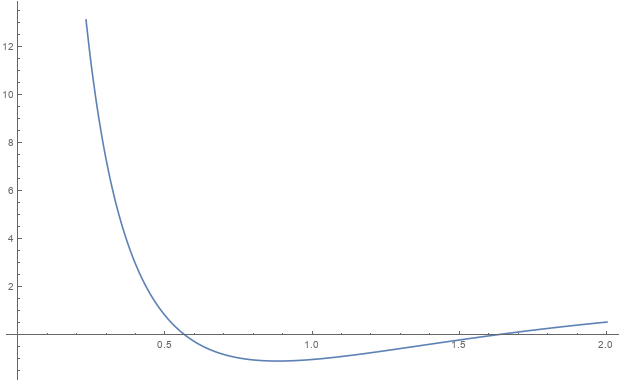
\includegraphics[scale=0.4]{graficaFalsa2.png}

\subsection{Hacer un programa que encuentre...}
Usé el mismo programa, sólo cambié la condición de paro y salen estos resultados:

\begin{center}
    \begin{tabular}{||c c c c c c c||} 
    \hline
    $n$ & $a$ & $b$  & $c$ & $f(a)|$ & $f(b)$ & $f(c)$ \\ [0.5ex] 
    \hline\
    0 & 0.55 & 0.57 & 0.5682478058  & 0.1807752434 &  -0.0173584340 & -0.0010583244\\ 
    \hline
    1 & 0.5682478058 & 0.57  & 0.5681340403  & -0.0010583244 & -0.0173584340 &  -0.0010583244 \\
    \hline
    2 & 0.5681340403 & 0.57  & 0.5681347676   & 0.0000067682& -0.0173584340  &  0.0000067682\\
    \hline
    3 & 0.5681347676  & 0.57  & 0.5681347629 &  -0.0000000433 &  -0.0173584340 & -0.0000000433\\
    \hline
    4 & 0.5681347629 & 0.57  & 0.5681347630 & 0.0000000003 &  -0.0173584340  & 0.0000000003[1ex]

   \end{tabular}
\end{center}

Para el método de biseccion tenemos 27 iteraciones.
Para el método de secante tenemos 5 iteraciones.

\begin{center}
    \begin{tabular}{||c c c c c c c||} 
    \hline
    $n$ & $a$ & $b$  & $c$ & $f(a)|$ & $f(b)$ & $f(c)$ \\ [0.5ex] 
    \hline\hline
    0 & 1.6 & 1.7 & 1.6096555585 & -0.0154930888 &  0.1449646285 & 0.0004520236\\ 
    \hline
    1 & 1.6096555585& 1.7  & 1.6093729685 & 0.0004520236 & 0.1449646285&  0.0004520236 \\
    \hline
    2 & 1.6093729685 & 1.7  & 1.6093813066  & -0.0000133387 & 0.1449646285  &  -0.0000133387\\
    \hline
    3 & 1.6093813066  & 1.7  & 1.6093810607 & 0.0000003935  &  0.1449646285 & 0.0000003935\\
    \hline
    4 & 1.6093810607 & 1.7  & 1.6093810679 & -0.0000000116 &  0.1449646285  & -0.0000000116\\
    \hline
    5 & 1.6093810679 & 1.7  & 1.6093810677 & 0.0000000003 &  0.1449646285  & 0.0000000003[1ex]

   \end{tabular}
\end{center}

Para el método de biseccion tenemos 29 iteraciones.
Para el método de secante tenemos 5 iteraciones.


\end{document}